\documentclass[journal,letterpaper]{article}

%Imports

\usepackage[utf8]{inputenc}
%headings
\usepackage{fancyhdr}
%double-space
\usepackage{setspace}
%\say command
\usepackage{dirtytalk}
%variable margins
\usepackage{geometry}
%make the margins a bit less ridiculous
\newgeometry{top=1in,bottom=1.5in,left=1in,right=1in}
%images
\usepackage{graphicx}
\pagestyle{fancy}

\usepackage{tikz}
\usetikzlibrary{arrows}


\title{Dream Design - Better Apple Watch}
\author{Edward Seim}


\begin{document}
    \maketitle
    
    \section{Introduction}
    \label{introduction}

    As an avid advocate of the Pebble Watch, the main thing that dissappoints me about the Apple Watch is the simplicity that is lost by bringing the complexity of iPhone apps to the watch screen. The root of this problem is the use of the touchscreen. As a Pebble user, which has only buttons to use the device with, it makes it possible to use the watch with minimal thought and once you've used it for a while, you can eve perform tasks without looking at it. My goal with my improved Apple Watch interface is to maximize use of the physical controls of the original to a more Pebblistic ideology.

    \begin{figure}[htbp]
        \centering
        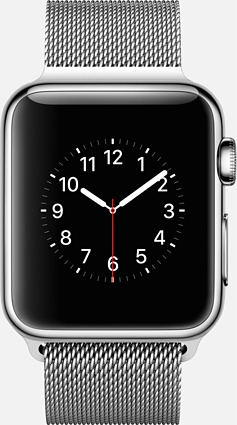
\includegraphics[width=10cm,height=10cm,keepaspectratio]{apple-watch}
        \caption{Apple Watch}
        \label{fig:apple_watch}
    \end{figure}

    \section{System}
    \label{System}

    Without any change to the hardware, the Apple Watch has the neccesary buttons to emulate a Pebble type simplicity. using the Digital crown as a select and scrolling mechanism, and the side button as the back button, you have the same capabilities as the Pebble Watch, with the better screen to display better eye candy.

    The most important change to the overall design of the interface is the change over to a menu type system. This means that the root level is the watch face. Hitting the Digital Crown will go into the main menu. Scrolling on this top menu will show the various different apps that you want use, for example the messaging or music apps. Hitting the back button will take you up a level in the menus. As a general principle, when there is content on the screen and scrolling lets you see more content while hitting the crown gives you the actions that can be performed in that context with that content. The actions will be sorted by highest use case. For example, in a text notification, the highest case would be \say{dismiss}, while the next option would be \say{reply}.

    An important thing to note is that at any point, the digital crown can be held down to bring up Siri, which can act upon the current content or anything in the global context.

    \section{Examples}
    \label{examples}

    \subsection{Message Notification}

    Fully fleshing out the idea presented earlier, we are looking at the case of recieving a message notification.

    In its natural state, Apple Watch is showing the main watchface. A message comes in and overlays over the watchface and indicates to the user that a notification has come in by firing off the Taptic Engine. Whats on the screen is something resembling the current Apple Watch, as seen in Figure \ref{fig:messages}. The dot next immediately next to the digital crown represents that there are actions that can be performed on this content. Figure \ref{fig:messages_actions} represents some of the actions that can be done on a message notification. Note that the \say{dismiss} option is currently selected. 

    Within a message notifcation, the Siri context includes things like dismiss and reply, where you can immediately dictate a responce by saying something like \say{Reply \say{I'll be home soon}}.

    \begin{figure}[htbp]
        \centering
        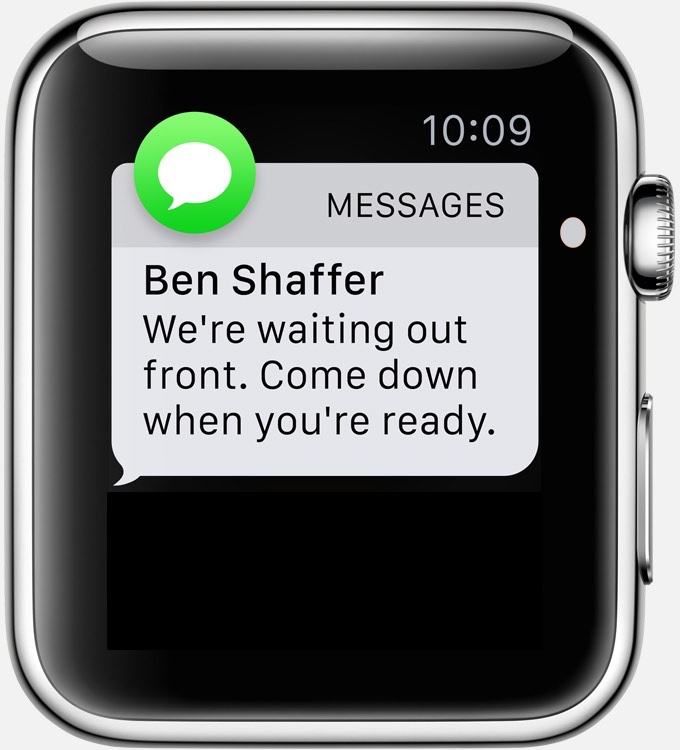
\includegraphics[width=10cm,height=8cm,keepaspectratio]{messages}
        \caption{Messages Main Content}
        \label{fig:messages}
    \end{figure}

    \begin{figure}[htbp]
        \centering
        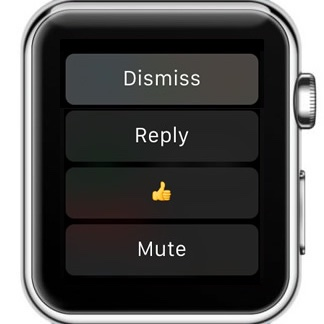
\includegraphics[width=10cm,height=8cm,keepaspectratio]{messages-actions}
        \caption{Messages Actions}
        \label{fig:messages_actions}
    \end{figure}

    \subsection{Music App}

    The Music app would be one of the apps listed in the top level menu directly beneath the watchface. You would see the song currently playing with corresponding artist and album names along with a playhead indicator and beautiful album artwork. Again, an indicator would be present next to the digital crown to indicate actions can be done on this content. The primary option would be to Play/Pause. Others would include volume and scrubbing, which would each present a vertical bar that can be manipulated with scrolling to get to the desired volume or playhead. Scrolling on the content, aka the currently playing song, would bring you to the full library. In this context, the actions that would be presented for this content would be different than that for the \say{Now Playing}. Things to change the view like sorting by artists, albums, or songs would be presented, along with the option for viewing playlsits.

    Within the Music App, the Siri context includes things like playing specific songs, artists, albums, playlists, along with changing the volume or playhead. For example, saying \say{Play songs by The Killers} would make Apple Watch start playback of songs by \say{The Killers} on the default listening interface. 

    \subsection{Yo App}
    
    Looking at a specific API, the Yo API seems the most applcable to a watch use because of its simplicity. This is something important to keep in mind with a watch application. Simplicity will mean you can get tasks done quickly and without much chance for user error.

    By opening the Yo app you have indicated that you wish to send a yo, as thats the only reason you would need to open the app. As such, the menu you are immediately presented with is the list of yo users you have configured already to send to. Simply scrolling to that user you wish to send a yo to and hitting the digital crown will prompt the sending of a yo to that user. The last option at the bottom of the list of users is an add button, which brings up Siri to dictate the user you wish to add.

    The Siri context within the Yo app includes performing actions like sending a yo to a specific user and adding a new user.

    \section{Rationale}
    \label{rationale}

    The most important part of the choice to go with the physical user controls rather than a touchscreen comes from the common usage locations of a watch. The original idea of a watch is to be able to be immediately check the time at any point. With the main watchface, the Apple Watch complications provide an at a glance view of the apps you care most about, all of which can be time adjusted with Time Travel, aka scrolling up or down while on the watchface. This lets you very quickly know whats coming up or behind you and what to look out for. Upon wanting to perform a task, its as close a single menu, where you have all your apps and terefore possible tasks listed out. If you want to contorl your music, theres an app for that. If you want to send a Yo, theres an app for that. Within each App, Siri pulls the appropriate context to make it quick to do any action without needing to do any digging. 

    The priority here is to make any task the user wants to complete or has to deal with be simple and quick so they can go back to the real world. at any content, the actions available are quickly accessable with one press of the digital crown. All this means that its very efficient to go from content to action. With the only user controls being the digital crown and the back button, learnability is easy and the control scheme is nicely uniform thorughout, preventing having \say{hidden features} or majorly unintuitive interfaces within apps. In the same way, memorabiltiy is high because you very quickly become accustomed to the actions you want to perform based on the content you have and can already know how much to scroll to get to the desired action. The only major error that would be posssible is not scrolling to the correct item in the menu you are viewing. This is averted from being a serious error by having a major indicator for the currently selected item. The physical pressing of the digital crown or the back button provide the affirmation of the action you have chosen.

    Watches are the kinds of items that should extend your abilities rather than consume your attention. This is what makes them less intrusive than smart phones. True satisfaction in a smartwatch comes from quickly performing tasks and getting back to what you were doing without getting drawn into something else. Content not allowing for such quick handling would therefore be dealt with by some other device, like a smartphone, tablet, or computer. 


\end{document}
